\section{Programmazione Concorrente}

\subsection{Multi-processo}
Un processo possiede: Il proprio PID (gestito dall'os), il PID del processo figlio o 0 e il pid del processo "iziale" (gestito da dscrittore di file). Comandi:

\begin{itemize}
	\item \textbf{fork()}  Crea un processo figlio. Condivide codice successivo alla fork e possiede una copia dei dati.

	Restituisce il pid del figlio al padre ($PID_F>0$) e 0 al figlio ($PID_F=0$) o un codice d'errore (<0).

	\item \textbf{exit(0)} Termina un processo restituendo lo stato indicato come parametro (0 stato successo).

	Se padre termina prima del figlio non si possono liberare le risorse.

	\item \textbf{wait(NULL)} Fa attendere al processo la terminazione del processo figlio. Restituisce il pid del processo terminato.

	\item \textbf{wait(pidProcesso)} Fa attendere al processo corrente uno specifico processo.

	\item \textbf{waitpid(pidProcesso, \&status, statoAttesso)} Fa aspettare un thread specifico con uno stato specifico.

	\item \textbf{exec} Sostituisce codice e dati a un processo. Non crea processi figlio.
\end{itemize}

Struttura base programma multi-processo:
\begin{verbatim}
						int main() {
							pid_t pid;

							pid = fork();

							if (pid<0) {"gestione errore"}
							else if (pid==0) {"processo figlio"}
							else {"processo padre"}
						}
\end{verbatim}

Ogni processo tiene referenza di un unico figlio, anche se ne può creare diversi. Quindi dopo ogni fork è buona cosa separare i flussi dei due processi.

\subsubsection{Comunicazione fra Processi (PIPE)}
Permette di comunicare fra processi correlati usando la funzione \textbf{pipe(nomePipe)} e i descrittori di file.
Esiste il collegamento fino a eliminazione esplicita o del processo.

Ogni processo ha un buffer di caratteri e una pipe (array di due celle) per scrivere e leggere con l'altro processo i dati contentuti nel buffer.

\begin{center}
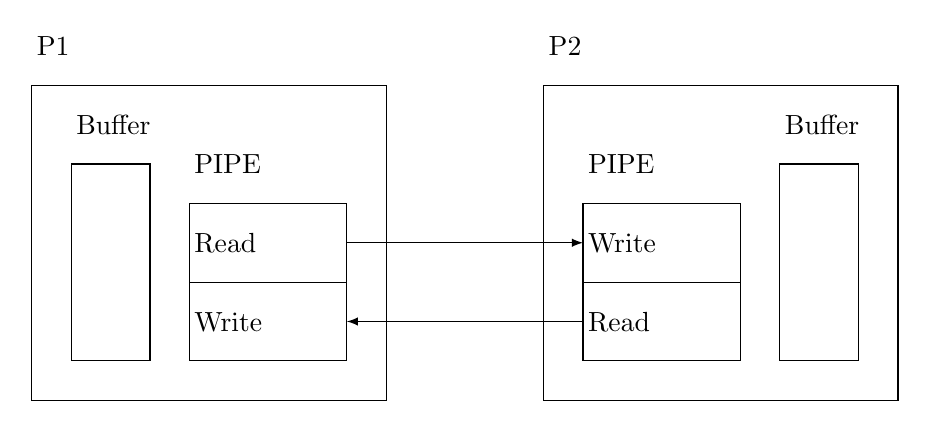
\begin{tikzpicture}
	\draw[draw=black, thin, solid] (-6.00,3.00) rectangle (-1.50,-1.00);
	\draw[draw=black, thin, solid] (-5.50,2.00) rectangle (-4.50,-0.50);
	\draw[draw=black, thin, solid] (-4.00,1.50) rectangle (-2.00,0.50);
	\draw[draw=black, thin, solid] (-4.00,0.50) rectangle (-2.00,-0.50);
	\node[black, anchor=south west] at (-6.06,3.25) {P1};
	\node[black, anchor=south west] at (-5.56,2.25) {Buffer};
	\node[black, anchor=south west] at (-4.06,0.75) {Read};
	\node[black, anchor=south west] at (-4.06,-0.25) {Write};
	\node[black, anchor=south west] at (-4.06,1.75) {PIPE};
	\draw[draw=black, thin, solid] (0.50,3.00) rectangle (5.00,-1.00);
	\draw[draw=black, thin, solid] (3.50,2.00) rectangle (4.50,-0.50);
	\draw[draw=black, thin, solid] (1.00,1.50) rectangle (3.00,0.50);
	\draw[draw=black, thin, solid] (1.00,0.50) rectangle (3.00,-0.50);
	\node[black, anchor=south west] at (0.44,3.25) {P2};
	\node[black, anchor=south west] at (3.44,2.25) {Buffer};
	\node[black, anchor=south west] at (0.94,1.75) {PIPE};
	\node[black, anchor=south west] at (0.94,0.75) {Write};
	\node[black, anchor=south west] at (0.94,-0.25) {Read};
	\draw[draw=black, -latex, thin, solid] (-2.00,1.00) -- (1.00,1.00);
	\draw[draw=black, -latex, thin, solid] (1.00,0.00) -- (-2.00,0.00);
\end{tikzpicture}
\end{center}

Comandi:
\begin{itemize}
	\item \textbf{pipe(varPipe[2] : int) : int} Crea una pipe unidirezionale.

	Su varPipe[0] si leggerà. Su varPipe[1] si scriverà.

	Restituisce -1 in caso di errore, 0 se creazione avviene con successo.
	\item \textbf{close(varPipe[0\textbar1])} Chiude una estremità della pipe.
	\item \textbf{read(varPipe[0], buffer, bufferSize)} Blocca esecuzione in attesa di dati da leggere.
	\item \textbf{strcpy(buffer, "...")} Prepara il buffer con il messaggio da inviare.
	\item \textbf{write(varPipe[1], buffer, sizeBuffer+1)} Scrive nella pipe.
\end{itemize}

Nota: I processi sono visti come file, per questo le operazioni si chiamano come quelle dei file.

\subsubsection{Inclusioni speciali}
\begin{itemize}
	\item \textbf{\#include <sys/types.h>} Definire tipi di dato speciali usati nelle chiamate di sistema.
	\item \textbf{\#include <unistd.h>} Include funzioni e costanti del sistema operativo Linux/Unix.
\end{itemize}

\subsection{Multi-thread}
\begin{itemize}
	\item \textbf{nomeFunzioneThread(arg : void*) : void*} Funzione assegnata da eseguire a un thread.

	Necessita questa firma specifica per accettare e restituire qualsiasi tipo di dato. Serve eseguire un cast esplicito.
	\item \textbf{pthread\_create(\&varThread, \&pthreadAttribut, tFunction, \&args)} Crea un nuovo thread dentro al processo corrente. I parametri sono:
	\begin{enumerate}
		\item Variabile tipo thread.
		\item Puntatore a struttura di attributi del thread. Default è NULL.
		\item Funzione che sarà eseguita dal thread.
		\item Puntatore a struttura contenente parametri usati dalla funzine.
	\end{enumerate}
	\item \textbf{pthread\_join(\&varThread, NULL)} Fa attendere processo la fine del thread indicato.
\end{itemize}

Struttura base programma multi-processo:
\begin{verbatim}
						void *tFunction(void *args) {...}
						int main() {
							pthread_t thread;
							... args = ...;

							ptread_create(&thread, NULL, tFunction, &args);
						}
\end{verbatim}

Nota: La creazione di un processo è più lenta della creazione di un thread perchè nella prima bisogna creare un intero file descriptor, mentre nella seconda parziale.